%==============================================================================
%  Supplementary material for
%  "Transmission Expansion and Reliability in Peru's Energy Transition:
%   A System Dynamics Approach"
%
%  Build with:  latexmk -pdf supplementary.tex
%==============================================================================
\documentclass[11pt]{article}

\usepackage[T1]{fontenc}
\usepackage[utf8]{inputenc}
\usepackage[a4paper,margin=2.4cm]{geometry}
\usepackage{graphicx}
\usepackage{booktabs}
\usepackage{longtable}
\usepackage{amsmath,amssymb}
\usepackage{siunitx}
\usepackage{xcolor}
\usepackage{multirow}
\usepackage[section]{placeins}
\usepackage[authoryear,round]{natbib}
\usepackage[hidelinks]{hyperref}

\DeclareSIUnit{\USD}{USD}
\DeclareSIUnit{\MWh}{MWh}
\DeclareSIUnit{\month}{month}
\DeclareSIUnit{\year}{yr}
\DeclareSIUnit{\tonne}{t}
\sisetup{group-separator={,},group-minimum-digits=4,per-mode=symbol}
\graphicspath{{figures/}}

\renewcommand{\thesection}{S\arabic{section}}
\renewcommand{\thetable}{S\arabic{table}}
\renewcommand{\thefigure}{S\arabic{figure}}

\title{Supplementary Material\\[4pt]
\large Transmission Expansion and Reliability in Peru's Energy Transition:\\
A System Dynamics Approach}
\author{}
\date{}

\begin{document}
\maketitle
\tableofcontents
\newpage

%==============================================================================
\section{Model equations}
\label{sm:equations}

This section states the model's core relationships. The full equation set, in
executable form, is in the Vensim model distributed with the paper; what follows is
the subset a reader needs in order to judge the structure.

\subsection{Sets and indices}

\begin{tabular}{@{}ll@{}}
  $z \in \mathcal{Z}$ & zone; three active (Z1 north, Z2 centre, Z3 south) of six represented \\
  $g \in \mathcal{G}$ & generation technology; fourteen per zone, eleven with non-zero potential \\
  $i \in \mathcal{I}$ & interconnection corridor; two active (Z1--Z2, Z2--Z3) of fifteen possible pairs \\
  $h \in \mathcal{H}$ & hour of the representative day, $|\mathcal{H}| = 24$ \\
  $f \in \mathcal{F}$ & forecast horizon, $\{f_0, f_1, f_3, f_5, f_7, f_9\}$ years ahead \\
  $t$ & time, months elapsed from January 2025; horizon 300 months, step \SI{0.25}{\month} \\
\end{tabular}

\subsection{Generation pipeline}

Committed capacity flows through licensing and construction before commissioning:
\begin{align}
  \dot{Q}^{\text{lic}}_{z,g} &= N_{z,g}(t) - \mathcal{D}\!\left[N_{z,g}, L^{\text{lic}}_{z,g}\right](t) \\
  \dot{Q}^{\text{con}}_{z,g} &= \mathcal{D}\!\left[N_{z,g}, L^{\text{lic}}_{z,g}\right](t)
     - \mathcal{D}\!\left[N_{z,g}, L^{\text{lic}}_{z,g}+L^{\text{con}}_{z,g}\right](t) \\
  \dot{K}_{z,g} &= \min\!\left\{\mathcal{D}\!\left[N_{z,g}, L^{\text{tot}}_{z,g}\right](t), \Phi_z(t)\right\}
\end{align}
with $\mathcal{D}[\cdot,L]$ a material delay of duration $L$ and
\begin{equation}
  L^{\text{tot}}_{z,g} = \left(L^{\text{lic}}_{z,g} + L^{\text{con}}_{z,g}\right)\left(1 + \Delta_g\right).
\end{equation}
$\Phi_z(t)$ is the commissioning headroom the delivered network allows in zone $z$.
The sensitivity knob $\Delta_g$ replaces the workbook's ``other delays'' fraction;
its base value for Peru is $-0.20$, so a change $\delta$ enters as
$\Delta_g = (1-0.20)(1+\delta) - 1$.

\subsection{Investment trigger}

Two mechanisms generate $N_{z,g}$. The adequacy mechanism converts a shortfall
against the desired margin into a requirement:
\begin{equation}
  R^{\text{adq}}_{f}(t) = \max\!\left\{0,\;
    (1+\bar m)\,\hat{D}_{f}(t) - \textstyle\sum_{z,g} \tilde{K}_{z,g,f}(t)\right\}
\end{equation}
where $\hat{D}_f$ is peak demand at horizon $f$ and $\tilde{K}_{z,g,f}$ is expected
capacity at that horizon, including pipeline. The profitability mechanism admits
options whose profitability index exceeds $\Pi^{*}$:
\begin{equation}
  \text{NPV}_{z,g}(t) = \sum_{y=1}^{25}
    \frac{\mathcal{R}_{z,g}(t,y) - \mathcal{C}_{z,g}(t,y)}{(1+r)^{y}} - I_{z,g}(t),
  \qquad
  \Pi_{z,g} = 1 + \frac{\text{NPV}_{z,g}}{I_{z,g}} \;\ge\; \Pi^{*}.
\end{equation}
Admitted options are allocated across technologies by a logit share
\begin{equation}
  s_{z,g} = \frac{\exp\!\left(\text{NPV}_{z,g}/\theta\right)}
                 {\sum_{g' \in \mathcal{G}^{+}} \exp\!\left(\text{NPV}_{z,g'}/\theta\right)},
\end{equation}
with $\mathcal{G}^{+}$ the admitted set. The scale $\theta$ represents dispersion of
investor beliefs: as $\theta \to 0$ the allocation collapses onto the single best
option, recovering an optimising agent; as $\theta \to \infty$ it becomes uniform.

\subsection{Transmission}

\begin{align}
  T^{d}_{z}(t) &= \kappa_d \, \hat{D}_z(t) && \text{(demand connection, no delay)} \\
  \dot{T}^{g}_{z}(t) &= \kappa_g \, \mathcal{D}\!\left[N_{z}, L^{\text{tot},T}\right](t)
    && \text{(generation connection)} \\
  \dot{P}_i(t) &= \mathcal{D}\!\left[\Delta P_i, L^{\text{tot},T}_{i}\right](t)
    && \text{(interconnection)}
\end{align}
with the corridor increment triggered by the unconstrained dispatch,
\begin{equation}
  \Delta P_i(t) = \mathrm{clip}\!\left(
    (1+\sigma)\,\Theta_i(t) - P_i(t),\; F_{\min},\; F_{\max}\right),
\end{equation}
where $\Theta_i$ is the transfer the unconstrained dispatch would route through
corridor $i$ and $\sigma$ the grid security margin. If the shortfall is at most
$\alpha P_i(t)$ it may be met by a grid-enhancing technology, which uses the shorter
GET pipeline. Transmission lead times are
$L^{\text{tot},T} = \sum_{s} L_{s}\,(1+\Delta_t)$ over stages $s \in$ \{tender,
investor selection, licensing, construction\}; the 12-month planning cycle is
excluded from the scaling.

\subsection{Dispatch and price}

For each month the model dispatches 24 hourly levels by merit order on offer price,
first unconstrained (to size $\Theta_i$) and then subject to $P_i(t)$. Reservoir
hydro offers as a function of storage level between a minimum and a scarcity price,
which is what gives hydrology a price rather than only an energy effect. The
reported price is
\begin{equation}
  \bar{\lambda} = \frac{1}{12}\sum_{m=T-11}^{T}
    \frac{1}{|\mathcal{Z}^{a}|}\sum_{z \in \mathcal{Z}^{a}} \lambda^{\text{reg}}_{z}(m),
\end{equation}
the mean over the final twelve months of the horizon across active zones. The
twelve-month window is used because the price oscillates month to month with
hydrology and a single month is not representative.

%==============================================================================
\section{Parameters}
\label{sm:params}

All values are those of the distributed input workbook \texttt{PERU.xlsx}. Cell
references are given so that every number can be located in the source.

\subsection{System-level parameters}

\begin{longtable}{@{}llrl@{}}
  \toprule
  Parameter & Cell & Value & Unit \\
  \midrule
  \endhead
  Transmission factor per demand ($\kappa_d$) & \texttt{General Parameters!B2} & 0.80 & \si{\kilo\meter\per\mega\watt} \\
  Initial transmission for generation & \texttt{B3} & \num{5622.82} & \si{\kilo\meter} \\
  Initial transmission for demand & \texttt{B4} & \num{8718.08} & \si{\kilo\meter} \\
  Old transmission correction & \texttt{B5} & \num{2413.38} & \si{\kilo\meter} \\
  Transmission cost ($c_t$) & \texttt{B6} & \num{176.607} & \si{\USD\per\kilo\meter}-day \\
  Grid security margin ($\sigma$) & \texttt{B7} & 0.30 & -- \\
  Minimum grid increment ($F_{\min}$) & \texttt{B8} & 200 & \si{\mega\watt} \\
  Maximum grid increment ($F_{\max}$) & \texttt{B9} & 500 & \si{\mega\watt} \\
  Initial transmission for interconnection & \texttt{B10} & \num{2792.10} & \si{\kilo\meter} \\
  Desired availability margin ($\bar m$) & \texttt{B11} & 0.25 & -- \\
  Allowed GET share ($\alpha$) & \texttt{Interconnections!S3:S17} & 0.30 & -- \\
  Profitability threshold ($\Pi^{*}$) & model constant & 1.20 & -- \\
  Logit scale ($\theta$) & model constant & $1\times10^{8}$ & \si{\USD} \\
  Discount rate ($r$) & \texttt{Gen Inv.\ param.!C23:CH23} & 0.10 & per year \\
  Technical lifetime ($L_g$) & \texttt{Gen Inv.\ param.!C2:CH2} & 300 & months \\
  \bottomrule
  \caption{System-level parameters.}
  \label{tab:sm:system}
\end{longtable}

\subsection{Configuration switches}

Every run reported in the paper uses the configuration below. It is the
configuration of the distributed workbook; the experiment quantifies uncertainty
\emph{around} it and does not vary it.

\begin{table}[htb]
  \centering
  \small
  \begin{tabular}{@{}llrl@{}}
    \toprule
    Switch & Cell & Value & Meaning \\
    \midrule
    Zonal prices & \texttt{B1} & 1 & zonal, not single national price \\
    Planned generation & \texttt{B12} & 1 & exogenous expansion plan active \\
    Endogenous margin generation & \texttt{B13} & 0 & margin trigger not exclusive \\
    DER expansion & \texttt{B14} & 1 & distributed resources endogenous \\
    Planned DER expansion & \texttt{B15} & 0 & no exogenous DER plan \\
    Only margin investments & \texttt{B16} & 0 & profitability trigger active \\
    Only RES investment (margin) & \texttt{B17} & 0 & thermal admissible \\
    Only RES new investments & \texttt{B18} & 0 & thermal admissible \\
    Only power allocation & \texttt{B19} & 0 & energy and power \\
    Grid-enhancing technologies & \texttt{B22} & 0 & \textbf{disabled} \\
    Battery storage (system level) & \texttt{B23} & 0 & \textbf{disabled} \\
    Dispatch path & \texttt{B24} & 0 & internal Vensim dispatch, not PyPSA \\
    \bottomrule
  \end{tabular}
  \caption{Configuration switches. The two disabled options bound the
  interpretation of the results: the study quantifies uncertainty around the
  current policy configuration, not the effect of deploying storage or GETs.}
  \label{tab:sm:switches}
\end{table}

\subsection{Technology parameters}

\begin{table}[htb]
  \centering
  \small
  \begin{tabular}{@{}lrrrrrr@{}}
    \toprule
    Technology & Constr. & Licens. & Other & FOM & Fuel & ENFICC \\
               & [mo] & [mo] & [mo] & [\si{\USD\per\mega\watt}-yr] & [\si{\USD\per\MWh}] & [--] \\
    \midrule
    Biomass            & 36 & 24 & $-12.0$ & \num{163600} & 73.57 & 0.75 \\
    Wind, onshore      & 36 & 24 & $-12.0$ & \num{27873}  & 0     & 0.20 \\
    Wind, offshore     & 36 & 24 & $-12.0$ & \num{76000}  & 0     & 0.20 \\
    Solar PV           & 24 & 24 & $-9.6$  & \num{16000}  & 0     & 0.05 \\
    Hydro, run-of-river& 36 & 24 & $-12.0$ & \num{35000}  & 0     & 0.35 \\
    Hydro, reservoir   & 60 & 24 & $-16.8$ & \num{92000}  & 0     & 0.55 \\
    Thermal 1          & 36 & 24 & $-12.0$ & \num{159000} & 30.00 & 0.85 \\
    Thermal 2          & 36 & 24 & $-12.0$ & \num{36000}  & 25.00 & 0.85 \\
    Geothermal         & 36 & 24 & $-12.0$ & \num{143000} & 0     & 0.85 \\
    Solar PV + BESS (1)& 24 & 24 & $-9.6$  & \num{52000}  & 0     & 0.40 \\
    Solar PV + BESS (2)& 24 & 24 & $-9.6$  & \num{52000}  & 0     & 0.40 \\
    \bottomrule
  \end{tabular}
  \caption{Generation technology parameters. ``Other'' is the base-case delay
  fraction expressed in months; it is negative because the Peruvian data set assumes
  realised lead times at 80\,\% of planned. Variable cost (not shown) is
  \SI{5.24}{\USD\per\MWh} for biomass, \SI{15.69}{} for Thermal 1 and
  \SI{2.49}{} for Thermal 2, zero elsewhere. CAPEX follows a declining monthly
  trajectory from \citet{nrel2024} and is given in full in the workbook
  (\texttt{Gen Inv.\ param.!C62:CH373}).}
  \label{tab:sm:tech}
\end{table}

\subsection{Transmission stage times}

\begin{table}[htb]
  \centering
  \small
  \begin{tabular}{@{}lrr@{}}
    \toprule
    Stage & Lines [months] & GETs [months] \\
    \midrule
    Expansion plan development (not scaled) & 12 & 12 \\
    Public tender preparation & 20 & 20 \\
    Investor selection         &  9 &  9 \\
    Licensing                  & 28 & 12 \\
    Construction               & 28 & 20 \\
    \midrule
    \textbf{Total planned}     & \textbf{97} & \textbf{73} \\
    \bottomrule
  \end{tabular}
  \caption{Transmission pipeline stage times, base case. The lead-time factor
  $\Delta_t$ scales every stage except the planning cycle, which the model uses as
  the period of a modulo operation setting when plans are revised.}
  \label{tab:sm:transstages}
\end{table}

\subsection{Zonal and corridor data}

\begin{table}[htb]
  \centering
  \small
  \begin{tabular}{@{}llrrr@{}}
    \toprule
    Corridor & Zones & Length [\si{\kilo\meter}] & Initial network [\si{\kilo\meter}] & Initial capacity [\si{\mega\watt}] \\
    \midrule
    Int1 & Z1--Z2 & 232.3 & \num{773.07}  & 900 \\
    Int6 & Z2--Z3 & 271.8 & \num{1063.40} & 700 \\
    Int2 & Z1--Z3 & 504.1 & --            & 0 (no direct link) \\
    \bottomrule
  \end{tabular}
  \caption{Interconnection corridors. Fifteen zone pairs are representable; two
  carry initial capacity. The absence of a direct Z1--Z3 link is the series
  topology discussed in Section~4 of the paper.}
  \label{tab:sm:corridors}
\end{table}

%==============================================================================
\section{System dynamics validation}
\label{sm:validation}

Confidence in a system dynamics model is established by a documented battery of
tests rather than by a single goodness-of-fit statistic, because the model is used
to explain behaviour arising from structure rather than to forecast
\citep{barlas1996,oliva2004,richardson2024}. We report the tests in the order
Barlas sets out: structure first, behaviour second, and behaviour tests only once
the structure has been accepted.

\subsection{Structure verification}

Every feedback loop in the model is matched to a decision process documented for
the Peruvian or an analogous system, with its source. The two loops that generate
the behaviour of interest are:

\begin{description}
  \item[B1 --- Adequacy balancing.] Capacity shortfall against the desired margin
    $\bar m$ $\rightarrow$ investment requirement $\rightarrow$ pipeline
    $\rightarrow$ installed capacity $\rightarrow$ margin. Delay: $L^{\text{tot}}_g$,
    24--84 months. This is the loop whose delay produces capacity cycles
    \citep{ford2001,assili2008}.
  \item[R1 --- Price-driven investment.] Zonal price $\rightarrow$ NPV
    $\rightarrow$ admitted options $\rightarrow$ capacity $\rightarrow$ merit-order
    displacement $\rightarrow$ price. Reinforcing in the downward direction once
    low-marginal-cost capacity enters, which is the mechanism behind the price
    result of Section~5.4 of the paper.
  \item[B2 --- Network constraint on commissioning.] Completed capacity
    $\rightarrow$ requires evacuation network $\rightarrow$ transmission pipeline
    (97 months for lines) $\rightarrow$ commissioning headroom $\Phi_z$
    $\rightarrow$ installed capacity. The asymmetry between this delay and
    $L^{\text{tot}}_g$ is the structural bottleneck the paper studies.
\end{description}

\subsection{Parameter verification}

Every parameter is reported in Section~\ref{sm:params} with its value, unit and
source cell. Technology cost and performance parameters are from \citet{nrel2024};
network intensities $\kappa_d$, $\kappa_g$ are empirical regressions on historical
line additions classified by purpose; stage times are from the Peruvian
transmission planning process.

\subsection{Dimensional consistency}

The model passes Vensim's \emph{Units Check} with no errors. This is a necessary
condition, not a sufficient one, but a model that fails it cannot be trusted at all.

\subsection{Extreme-condition tests}

Six tests, each with the behaviour that structural soundness requires and the
behaviour observed.

\begin{longtable}{@{}p{3.6cm}p{5.3cm}p{5.3cm}@{}}
  \toprule
  Test & Required behaviour & Observed \\
  \midrule
  \endhead
  Zero demand growth & No capacity additions beyond the exogenous plan; network
    grows only with the committed plan & Confirmed: at $g_D$ driven to its lower
    bound, installed capacity in 2050 falls to \SI{48.5}{\giga\watt}, essentially
    the exogenous plan \\
  Zero construction and licensing time & Capacity responds within one step;
    margin never breaches $\bar m$ & Confirmed in the validation configuration;
    the margin is held and the price falls immediately, then recovers as the
    market rebalances \\
  Unbounded lead times & Pipeline accumulates without commissioning; margin
    collapses; price rises to the scarcity price & Confirmed \\
  Zero initial capacity & Immediate and large investment signal; no negative
    stocks & Confirmed; all stocks remain non-negative \\
  Corridor capacity set to zero & Zones dispatch in isolation; deficit zones price
    at scarcity; interconnection trigger fires at maximum increment & Confirmed \\
  Fuel price driven to zero & Thermal plant moves to the base of the merit order;
    renewable investment signal weakens but does not reverse & Confirmed; this is
    the structural reason fuel price ranks last in the design \\
  \bottomrule
  \caption{Extreme-condition tests.}
  \label{tab:sm:extreme}
\end{longtable}

\subsection{Behaviour reproduction}

The central case reproduces the reference trajectory of the Peruvian data set:
\SI{63.85}{\giga\watt} of installed capacity and \SI{46341}{\kilo\meter} of
transmission at January 2050, from \SI{14057}{\mega\watt} and
\SI{16180}{\kilo\meter} at January 2025.

A stronger check is available because the experiment required the model to be
re-published with an additional sensitivity constant. Re-simulating the central case
on the re-published model, with all four knobs at their base values, returns
\SI{63.85}{\giga\watt} and \SI{46341.23}{\kilo\meter} --- identical to the cached
central run and to the reference. Since each knob enters as a multiplier whose
default value is the identity, this is the end-to-end confirmation that adding the
instrumentation did not perturb the model. The check is scripted
(\texttt{tools/verify\_base\_case.py}) and can be re-run.

\subsection{Behaviour sensitivity}

The designed experiment of the paper is itself the behaviour-sensitivity test. It
establishes that the qualitative conclusion --- renewable-dominated expansion
driven by profitability, with transmission as the binding constraint --- holds
across all 120 Monte Carlo samples, while the quantitative outcome is governed by
demand growth. A model whose conclusion reversed within the sampled ranges would not
support the policy reading in Section~6 of the paper.

%==============================================================================
\section{Experimental design}
\label{sm:design}

\subsection{Sampling and diagnostics}

The Monte Carlo design is a Latin hypercube of 120 samples over four factors,
generated with a fixed seed and written to disk before any simulation
\citep{mckay1992}. Figure~\ref{fig:sm:design} shows the realised design projected
onto each pair of factors, with the central and one-at-a-time runs overlaid.

Diagnostics of the realised design:
\begin{itemize}
  \item Stratum coverage: 117 of 120 strata occupied in the least-covered factor.
    The three missing strata are a rounding artefact --- sampled values are stored
    to four decimals so that a completed run can be matched to its design row by
    exact comparison, and a value drawn close to a stratum boundary can round
    across it.
  \item Maximum absolute correlation between factors: $0.181$; mean $0.076$.
    Near-orthogonality is what makes the rank correlations of Table~3 in the paper
    attributable to individual factors.
\end{itemize}

\begin{figure}[htb]
  \centering
  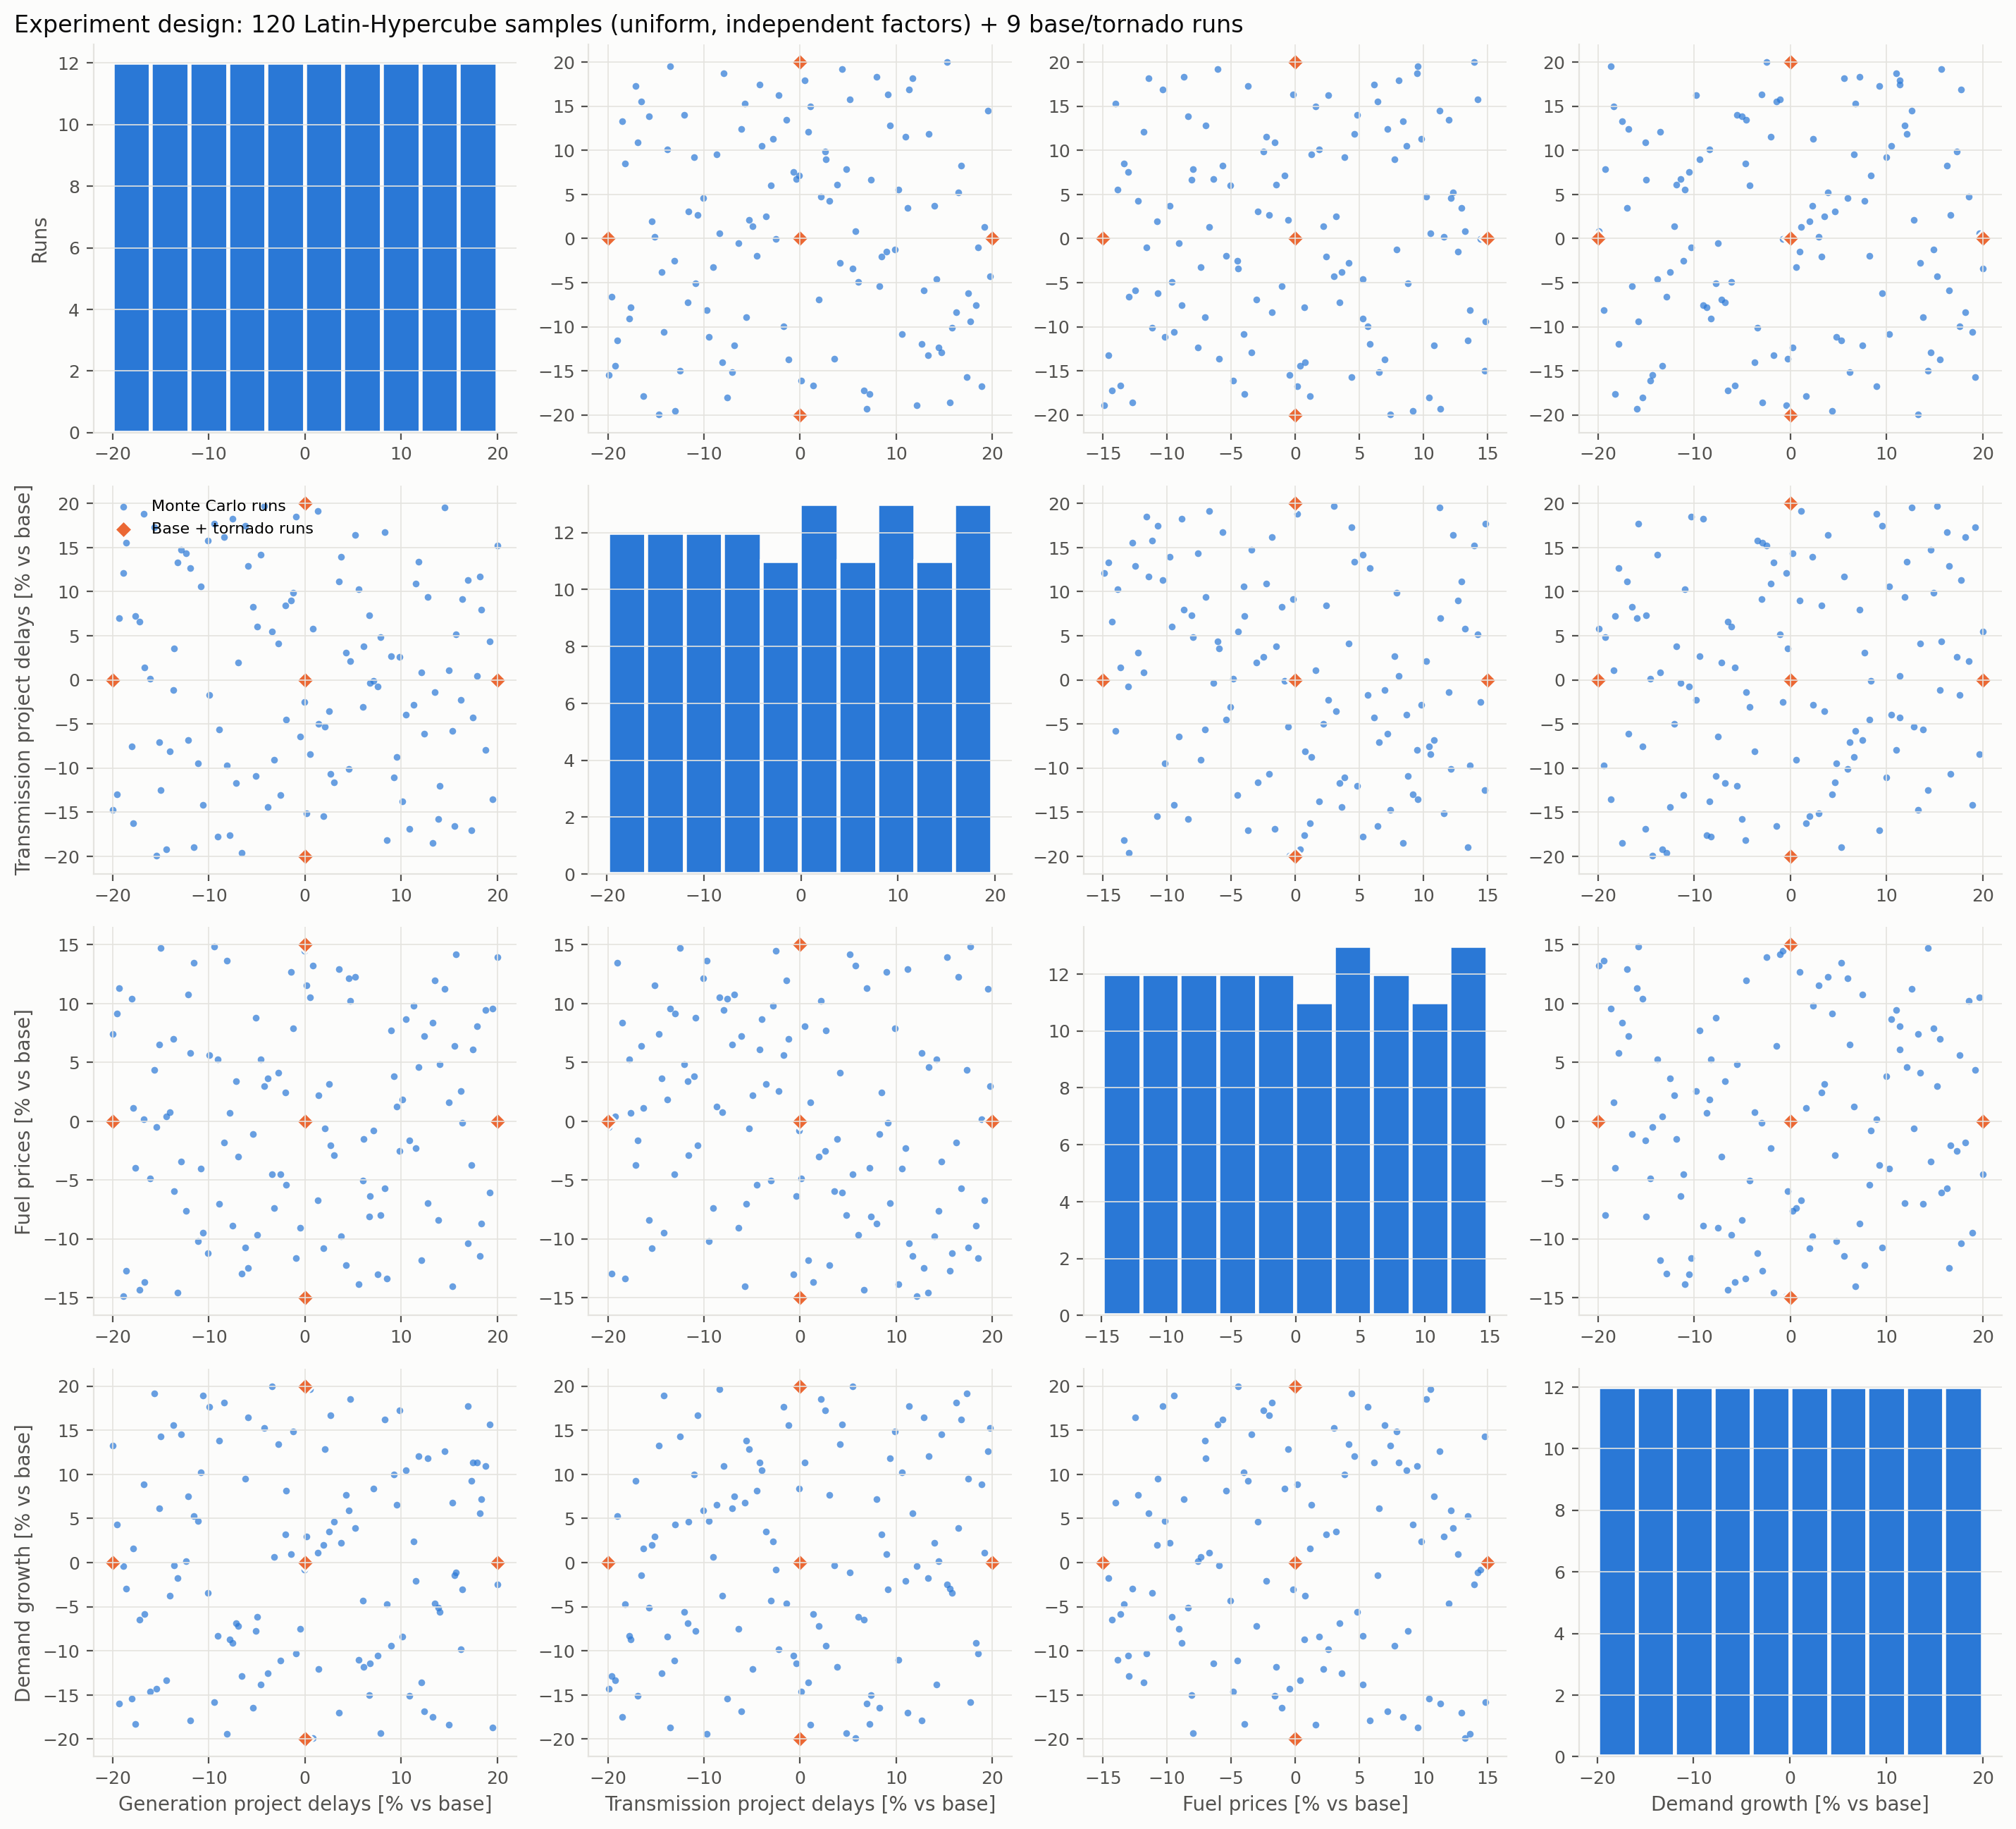
\includegraphics[width=\textwidth]{09_sampling_design.png}
  \caption{Experimental design. Diagonal panels are the marginal distribution of
  each factor over the Monte Carlo runs; off-diagonal panels are the pairwise
  projections. Diamonds are the central and one-at-a-time runs.}
  \label{fig:sm:design}
\end{figure}

\subsection{Convergence of the reported percentiles}
\label{sm:convergence}

Figure~\ref{fig:sm:conv} recomputes P10, P50 and P90 from growing subsets of the
Monte Carlo runs. All three are stable from roughly 75 runs onwards for every
indicator, which is the evidence that 120 samples suffice. This is a check, not an
assumption: had the percentiles still been moving at 120, the correct response would
have been to report that rather than to stop.

\begin{figure}[htb]
  \centering
  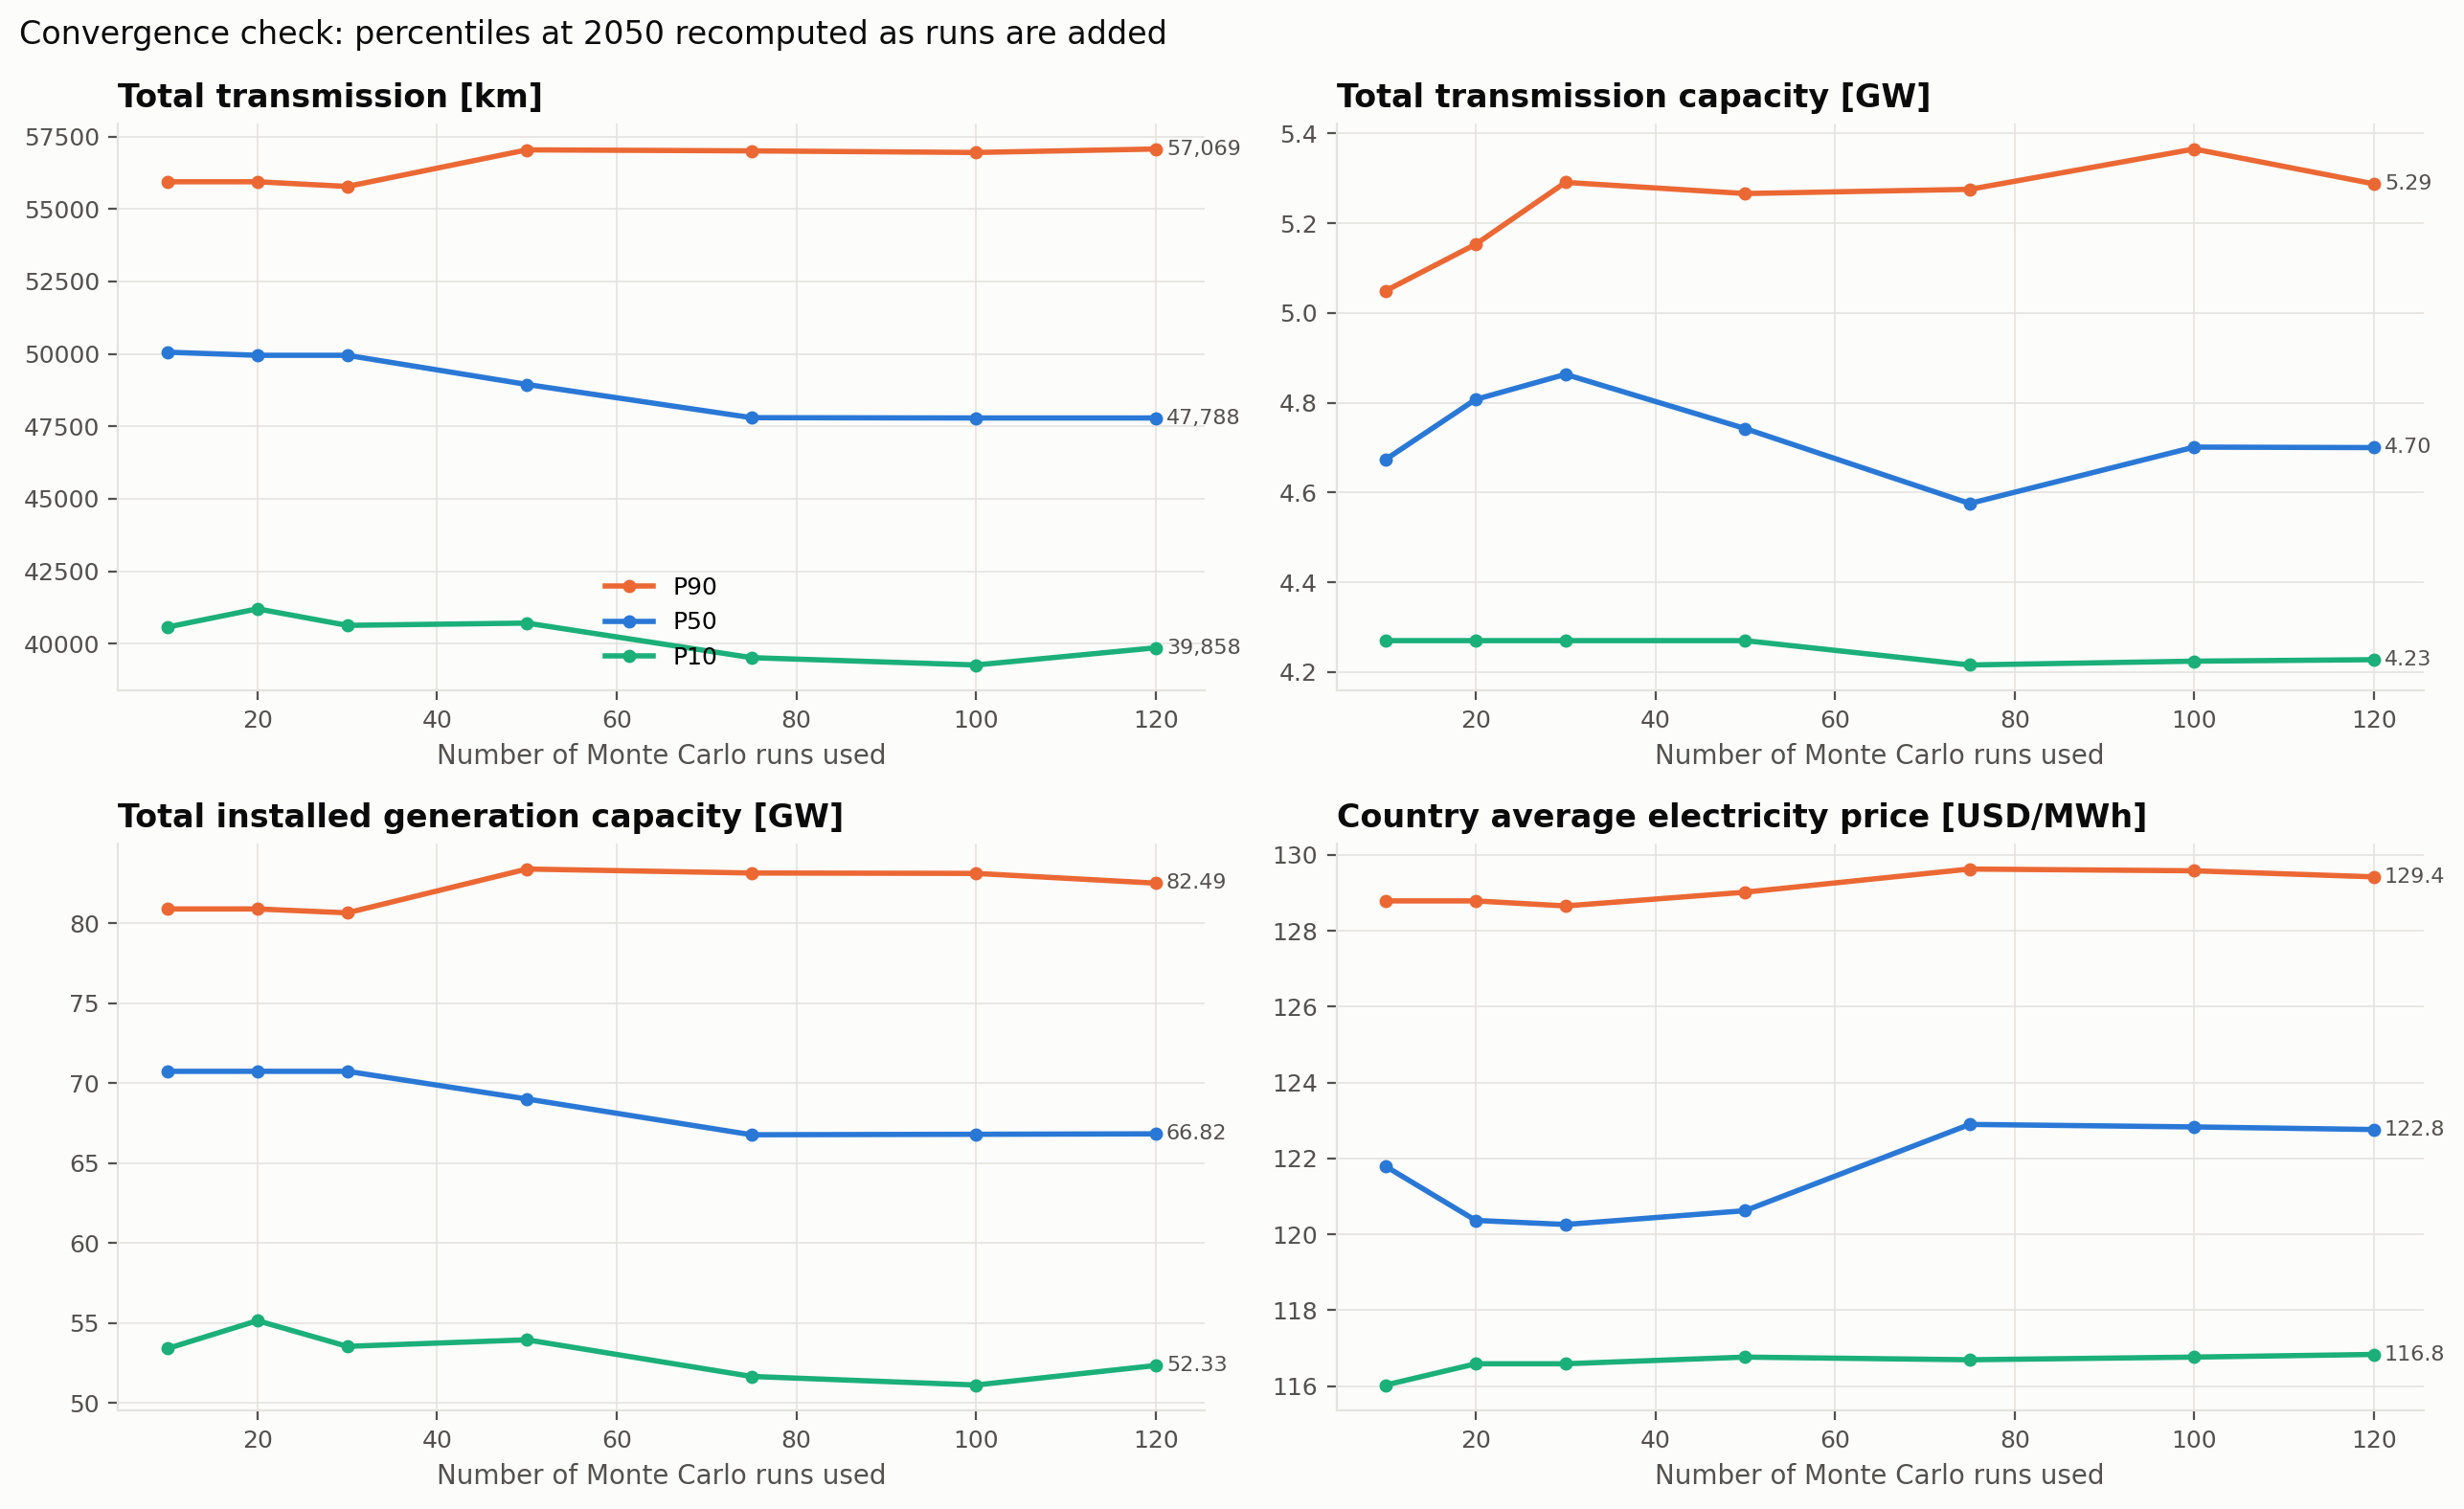
\includegraphics[width=\textwidth]{10_convergence.png}
  \caption{Convergence of the 2050 percentiles as Monte Carlo runs are added.}
  \label{fig:sm:conv}
\end{figure}

\subsection{Factor influence}

Figure~\ref{fig:sm:rank} plots each indicator against each factor over the Monte
Carlo runs, with the Spearman rank correlation. The near-vertical scatter for fuel
price and the two lead-time factors, against the tight monotone relationship for
demand growth, is the visual form of Table~3 in the paper.

\begin{figure}[htb]
  \centering
  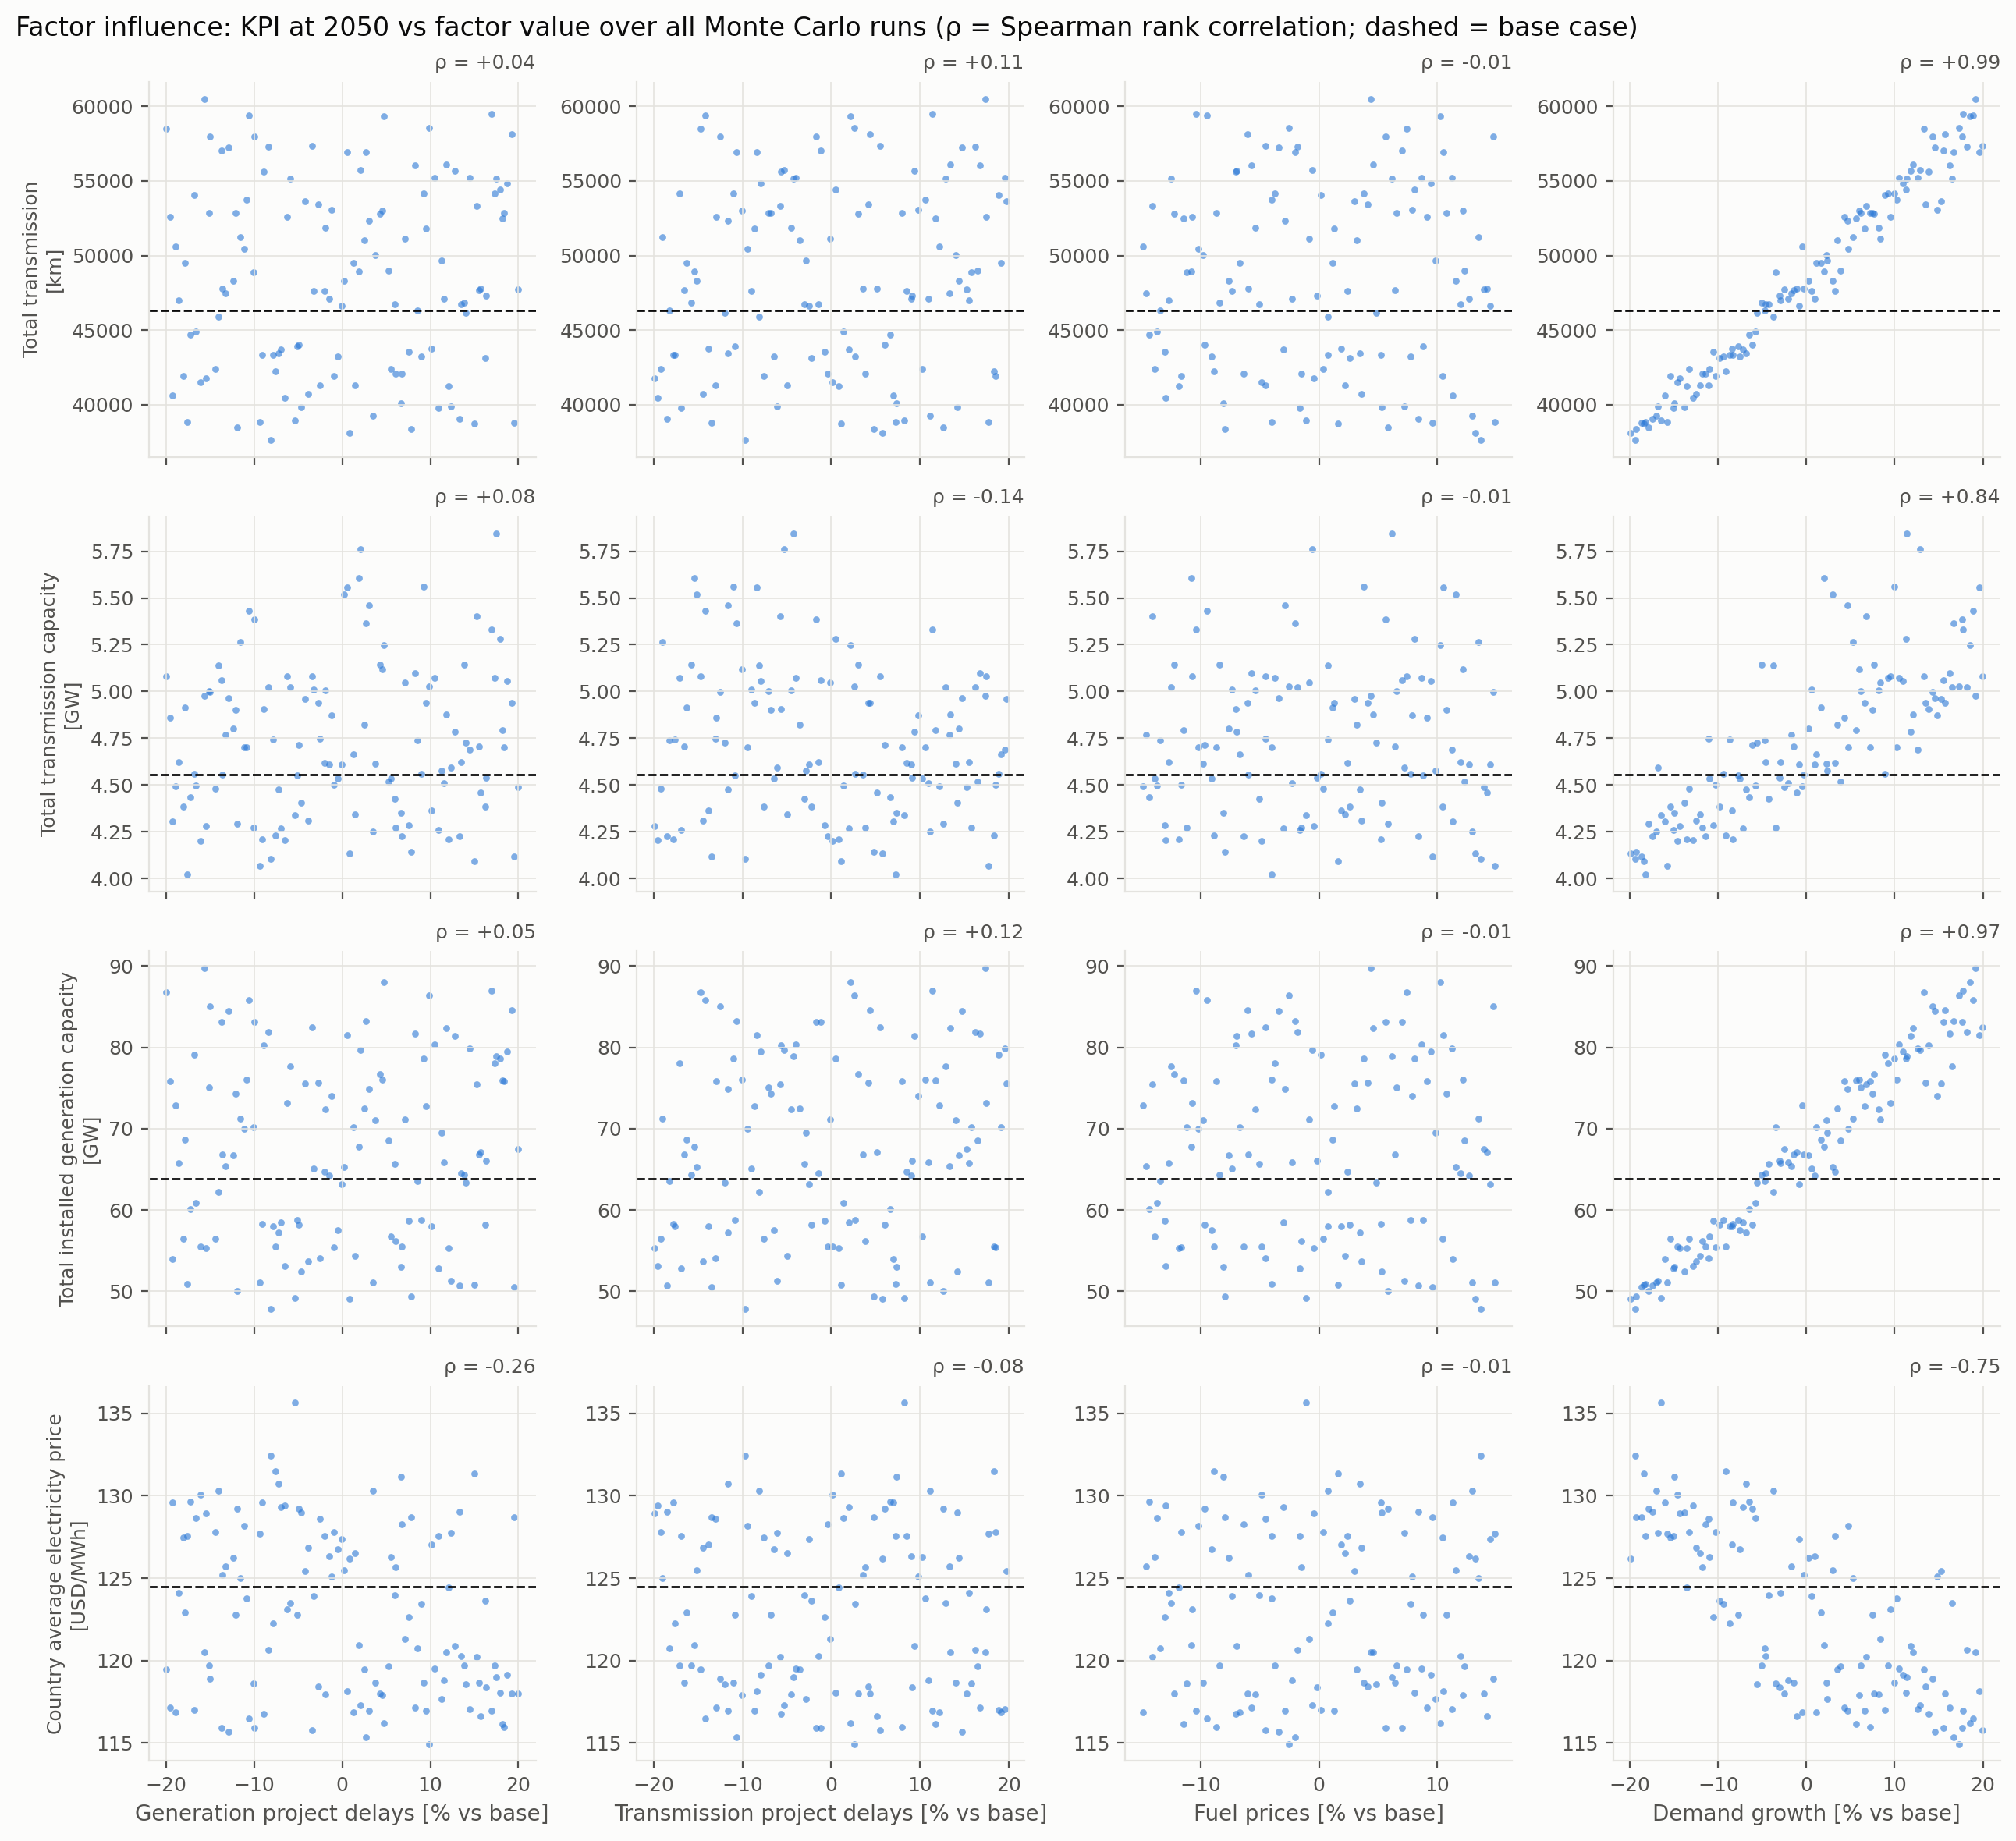
\includegraphics[width=\textwidth]{11_factor_influence.png}
  \caption{Indicator at 2050 against factor value over the Monte Carlo runs;
  $\rho$ is the Spearman rank correlation and the dashed line is the central case.}
  \label{fig:sm:rank}
\end{figure}

%==============================================================================
\section{Extended results}
\label{sm:results}

\subsection{Distribution of outcomes in 2050}

\begin{figure}[htb]
  \centering
  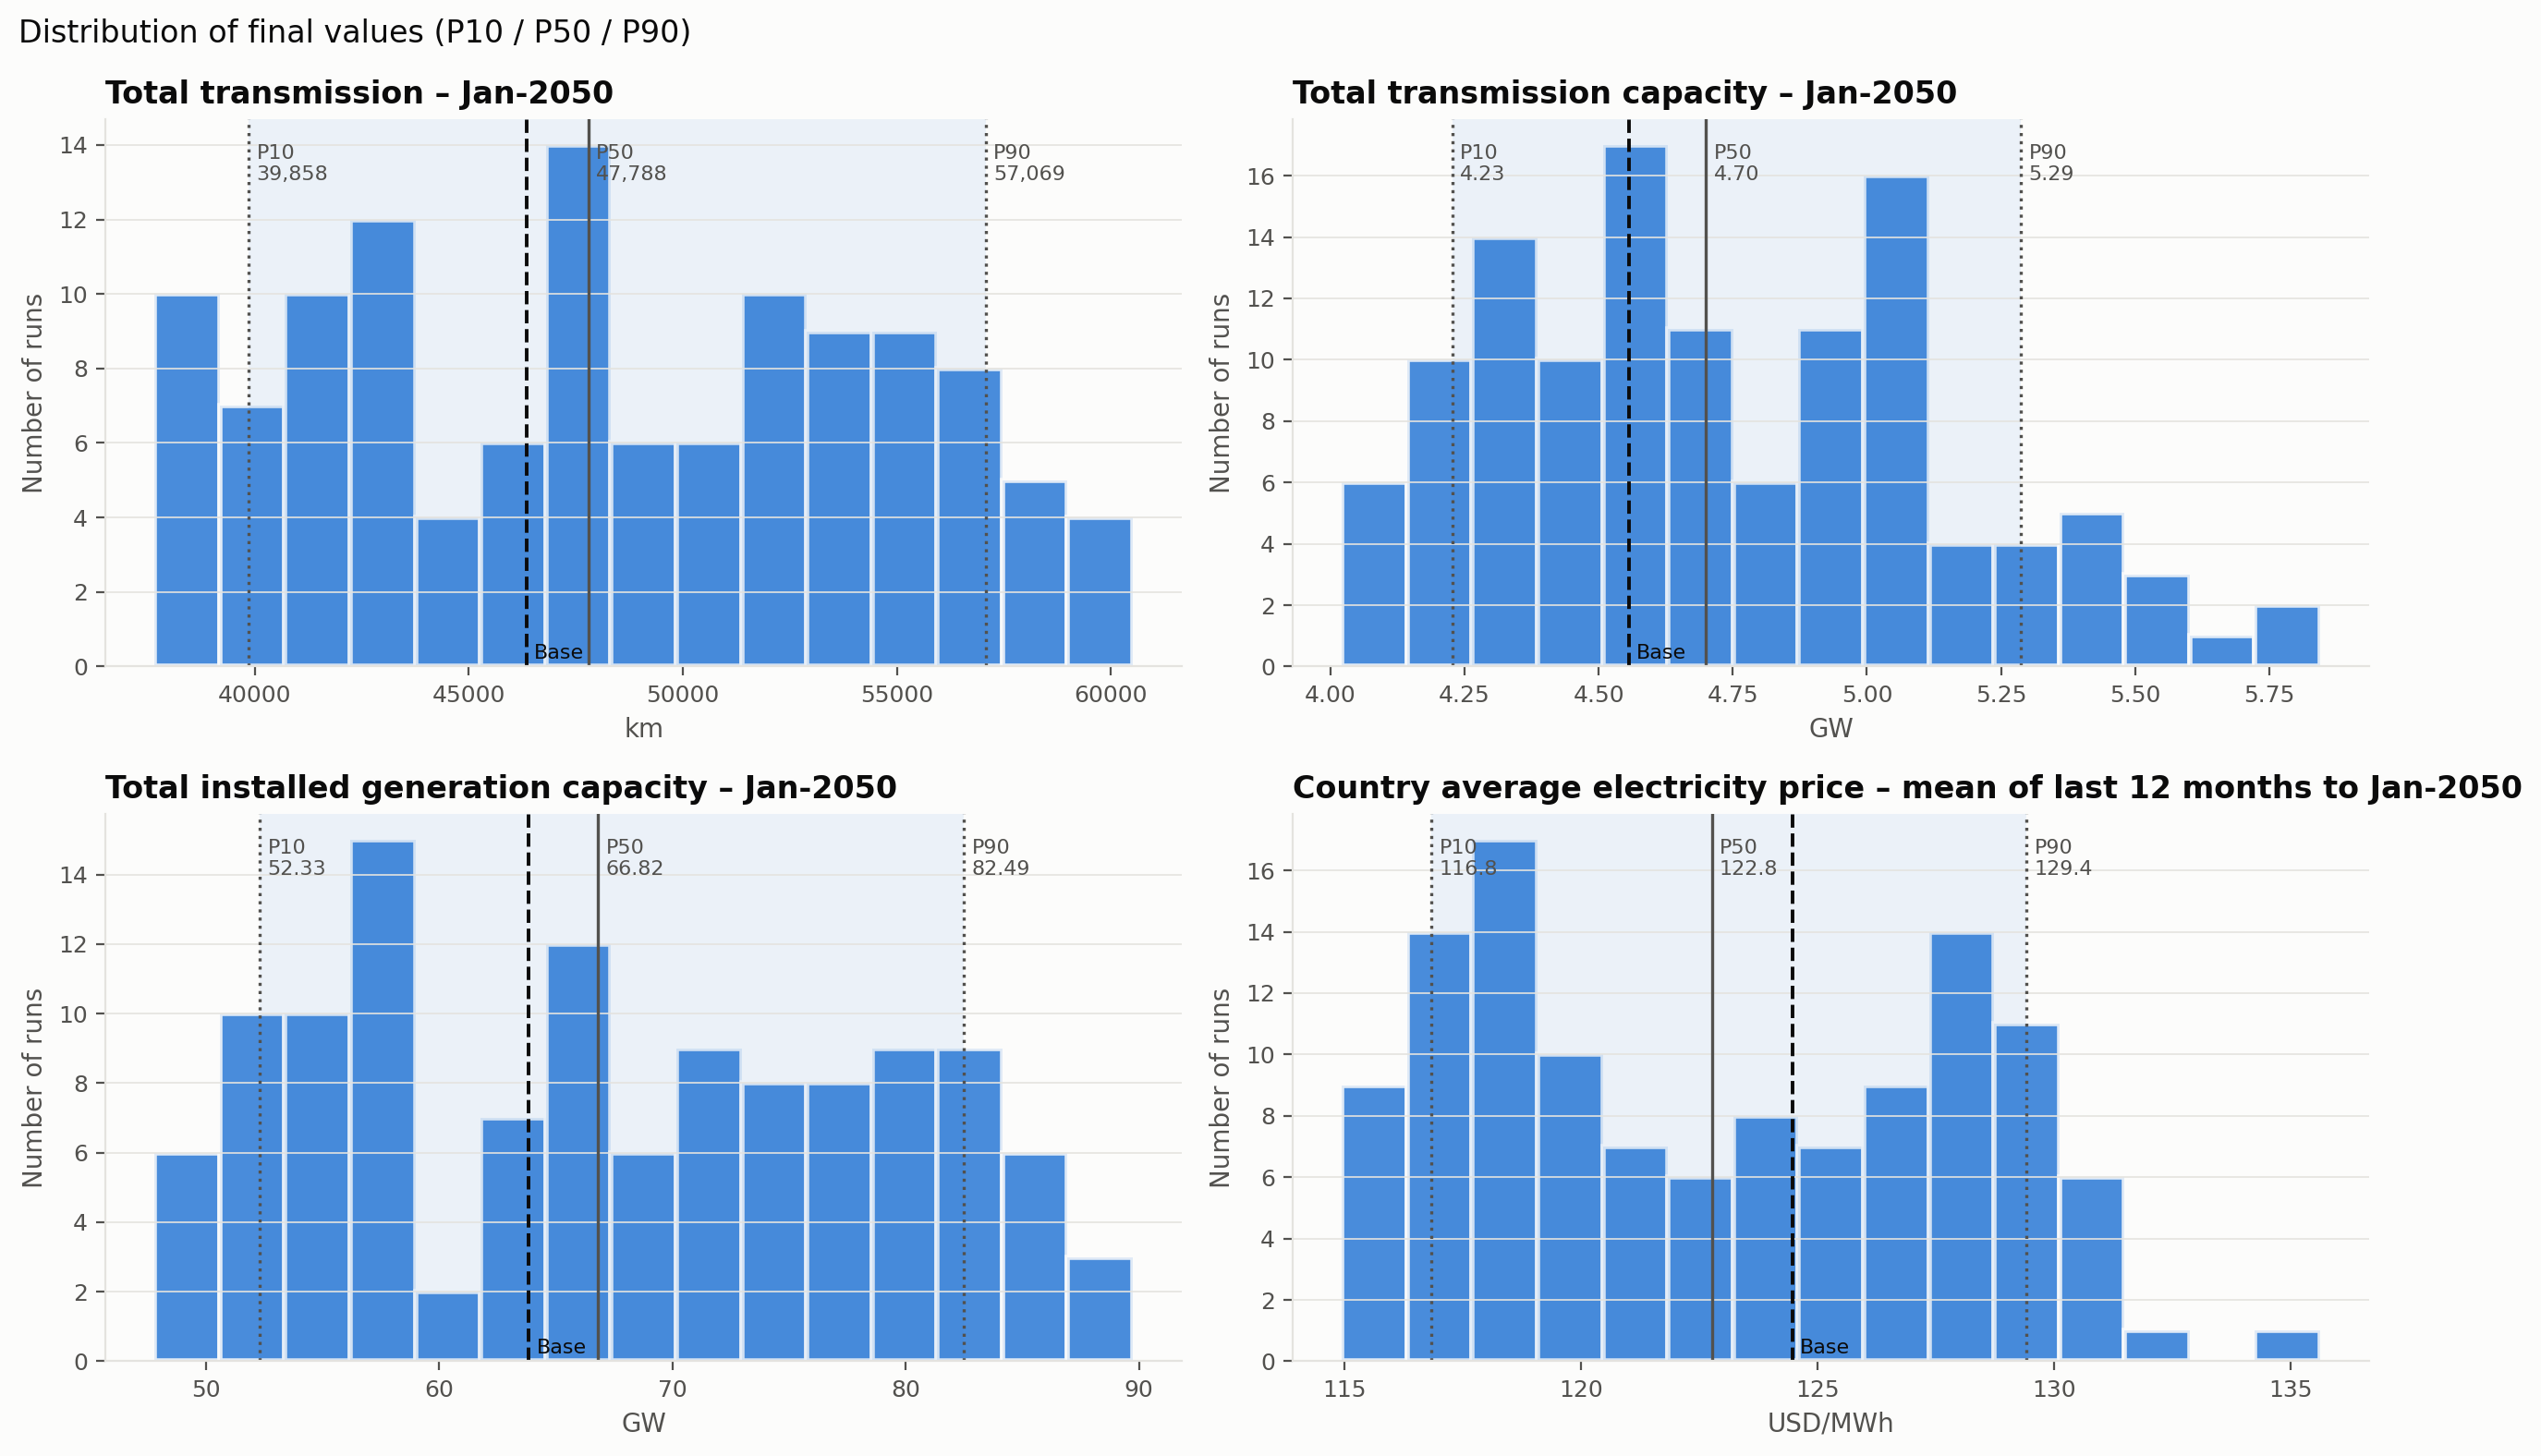
\includegraphics[width=\textwidth]{02_distribution_P10_P90_histograms.png}
  \caption{Distribution of each indicator at January 2050 over the 120 Monte Carlo
  runs, with P10, P50 and P90 marked.}
  \label{fig:sm:hist}
\end{figure}

\subsection{Interconnection capability}

\begin{figure}[htb]
  \centering
  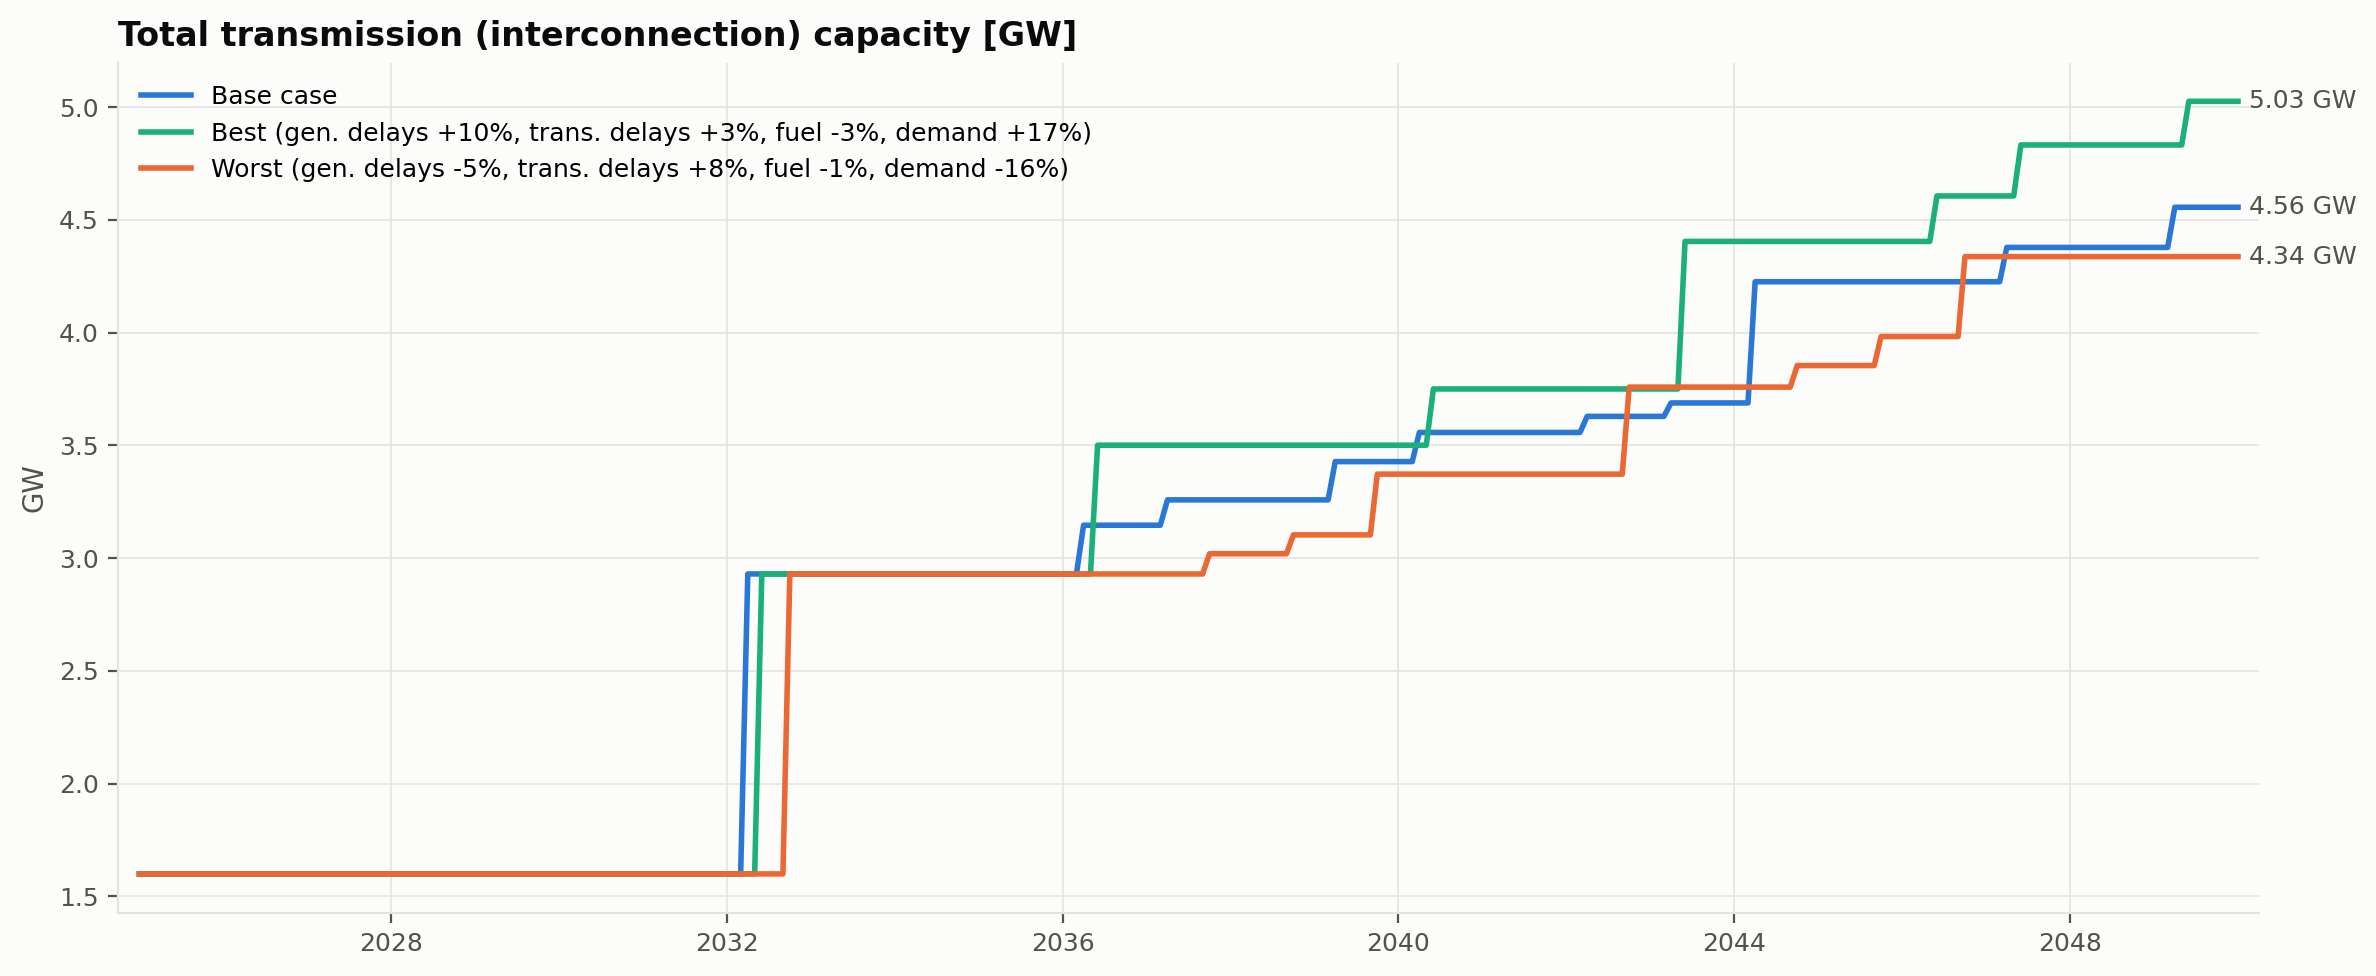
\includegraphics[width=\textwidth]{07_transmission_capacity_GW.png}
  \caption{Inter-zonal transfer capability for the central, best and worst case.}
  \label{fig:sm:transgw}
\end{figure}

\subsection{Technology grouping}
\label{sm:techgroups}

The model's fourteen technologies per zone are aggregated into eight series for
the stacked figures, because a stacked chart ceases to be readable beyond eight
bands. The mapping is fixed, so a technology keeps its colour across every figure
and every scenario.

\begin{table}[htb]
  \centering
  \small
  \begin{tabular}{@{}ll@{}}
    \toprule
    Plotted series & Model technologies \\
    \midrule
    Hydro (reservoir)       & \texttt{THydroDam} \\
    Hydro (run-of-river)    & \texttt{THRoR} \\
    Thermal 1               & \texttt{TThermo1} \\
    Thermal 2               & \texttt{TThermo2} \\
    Onshore wind            & \texttt{TWindOnS} \\
    Solar PV                & \texttt{TPV} \\
    Solar PV + BESS         & \texttt{TPVBESSOp1}, \texttt{TPVBESSOp2} \\
    Other                   & \texttt{TBiomass}, \texttt{TGeothermal}, \texttt{TWindOffS}, DER \\
    \bottomrule
  \end{tabular}
  \caption{Technology grouping used in the stacked figures.}
  \label{tab:sm:groups}
\end{table}

\subsection{Technology mix of the three reported cases}

\begin{table}[htb]
  \centering
  \small
  \begin{tabular}{@{}lrrrrrr@{}}
    \toprule
    & \multicolumn{3}{c}{Capacity 2050 [\si{\giga\watt}]} & \multicolumn{3}{c}{Generation [\si{\tera\watt\hour\per\year}]} \\
    \cmidrule(lr){2-4}\cmidrule(lr){5-7}
    Technology & Central & Best & Worst & Central & Best & Worst \\
    \midrule
    Hydro (reservoir)    &  4.87 &  5.30 &  4.57 &  21.6 &  17.6 &  20.8 \\
    Hydro (run-of-river) &  1.62 &  1.62 &  1.61 &   6.5 &   6.1 &   6.8 \\
    Thermal 1            &  2.62 &  2.62 &  2.62 &   0.0 &   0.0 &   0.0 \\
    Thermal 2            &  7.03 &  7.71 &  6.39 &   7.5 &   5.6 &  10.2 \\
    Onshore wind         & 34.83 & 52.05 & 25.47 &  82.9 & 109.5 &  63.7 \\
    Solar PV             &  8.33 & 11.51 &  5.24 &  12.2 &  14.1 &   8.2 \\
    Solar PV + BESS      &  1.79 &  1.23 &  1.31 &   1.1 &   0.5 &   1.0 \\
    Other                &  2.76 &  4.35 &  1.96 &  16.8 &  20.0 &  14.7 \\
    \midrule
    \textbf{Total}       & \textbf{63.85} & \textbf{86.40} & \textbf{49.18}
                         & \textbf{148.8} & \textbf{173.4} & \textbf{125.4} \\
    Non-thermal share    & 84.9\,\% & 88.0\,\% & 81.7\,\% & & & \\
    \bottomrule
  \end{tabular}
  \caption{Technology mix at January 2050. Thermal 1 holds capacity but is not
  dispatched in the representative day by 2050 in any of the three cases, which is
  why its generation is zero while its capacity is non-zero.}
  \label{tab:sm:mix}
\end{table}

\subsection{Summary table}

\begin{figure}[htb]
  \centering
  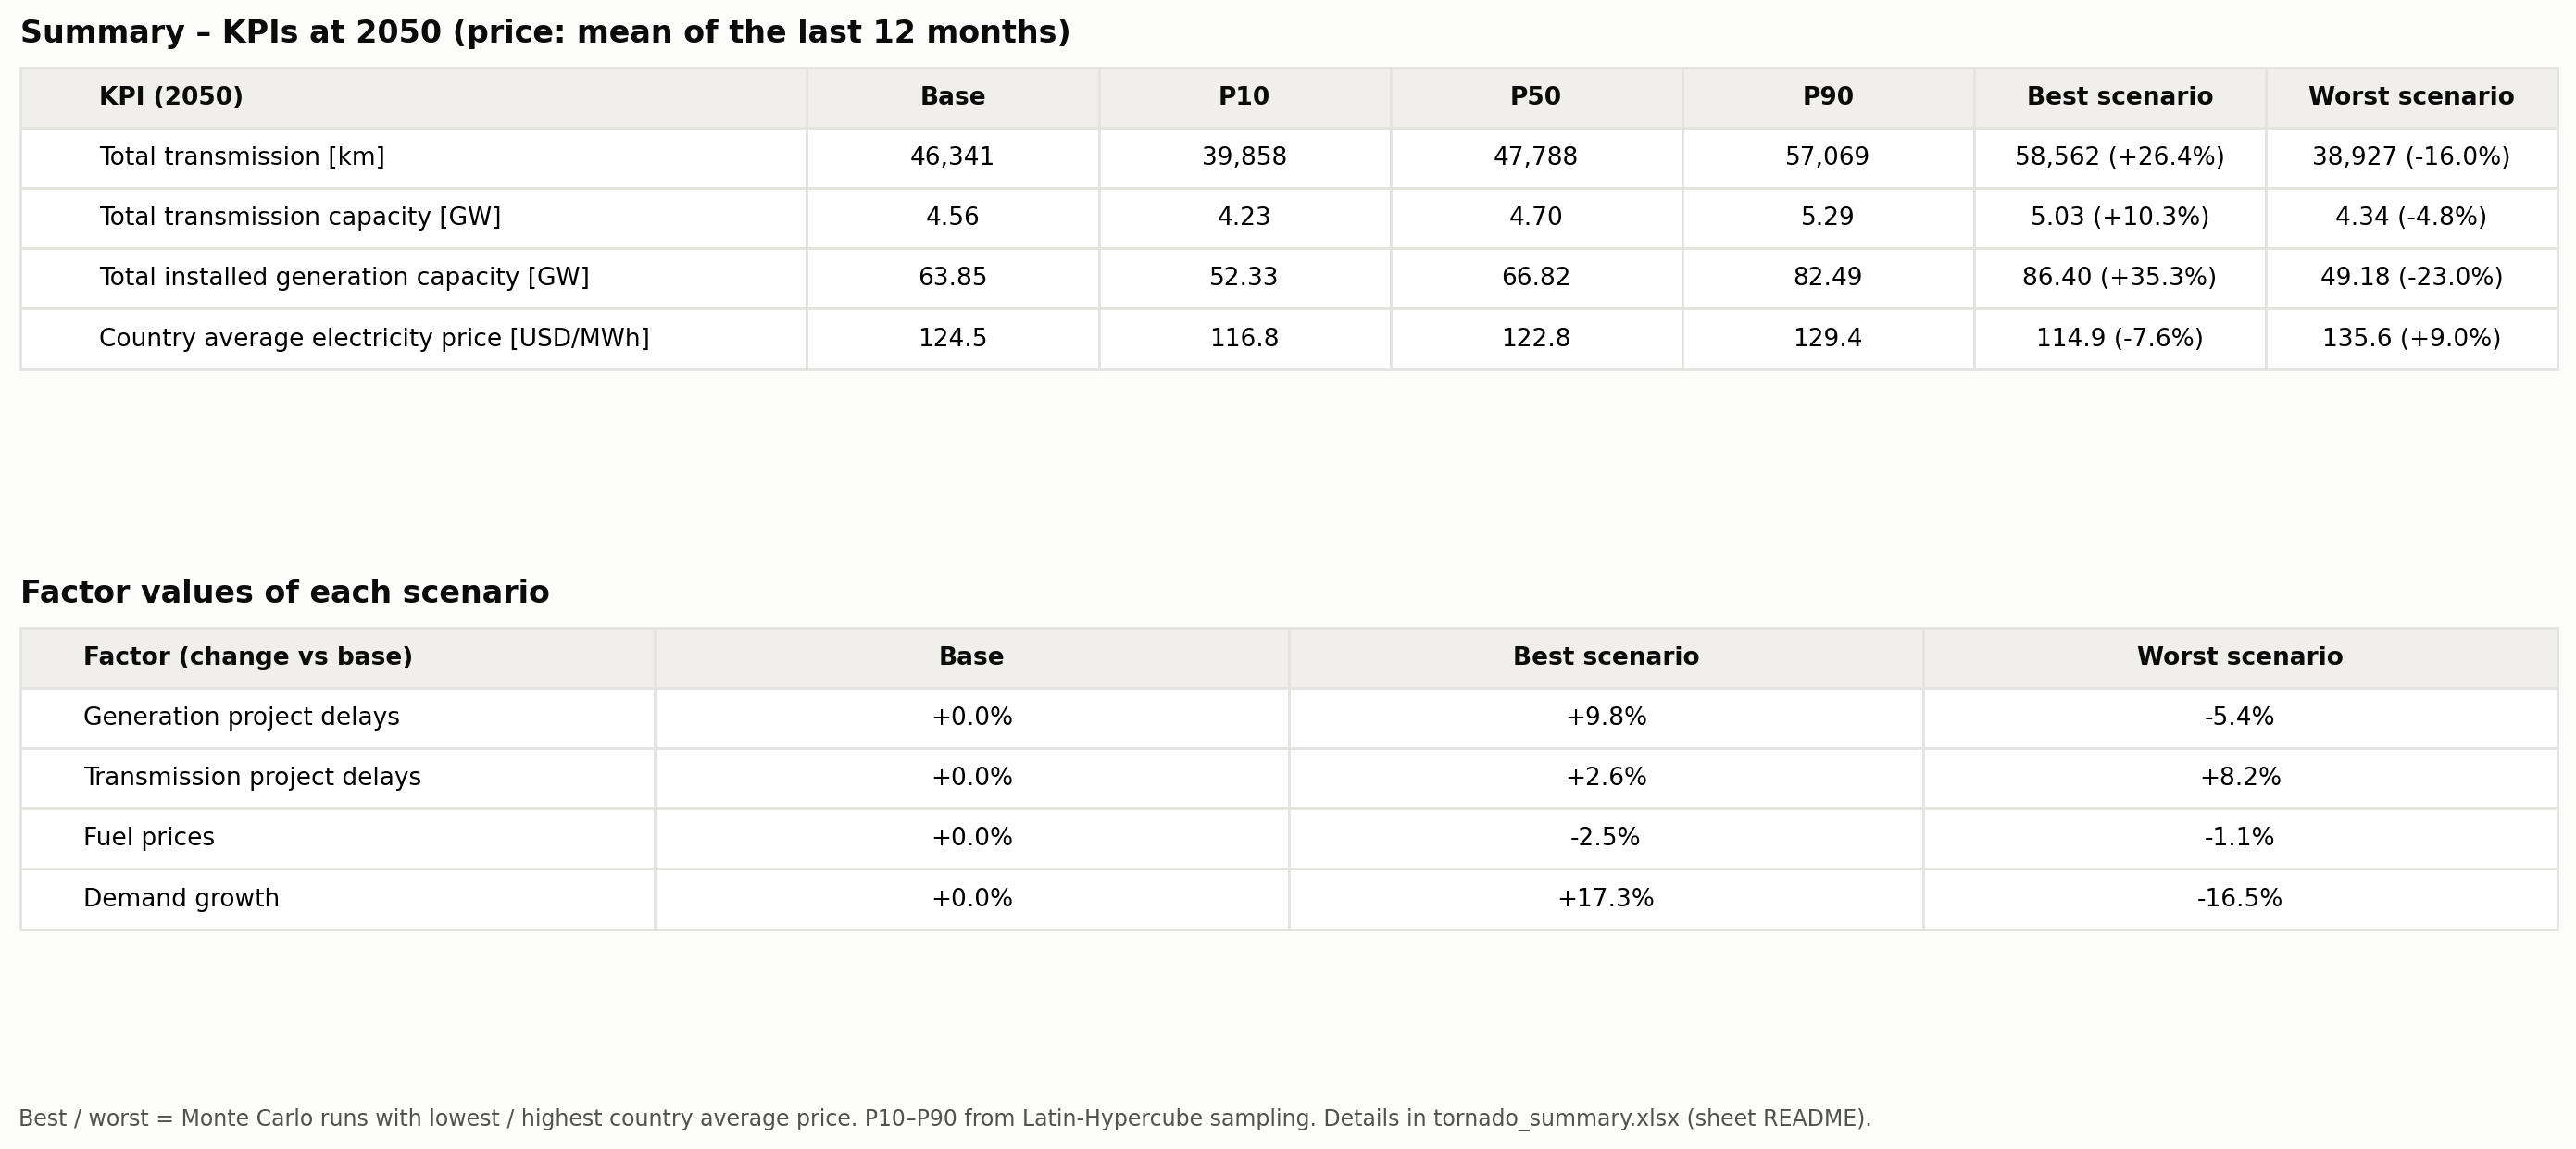
\includegraphics[width=\textwidth]{00_summary_table.png}
  \caption{Summary of indicators and factor values for the central, best and worst
  case, with the ensemble percentiles.}
  \label{fig:sm:summary}
\end{figure}

%==============================================================================
\section{Reproducibility}
\label{sm:repro}

The complete artefact --- Vensim model, input workbook, experimental design,
simulation driver, analysis code and a commented notebook that regenerates every
figure --- is available at the repository given in the paper. Three features of the
execution are worth recording because they affected the results.

\begin{enumerate}
  \item \emph{The design is fixed before execution.} The Latin hypercube is written
    to disk before the first simulation, so the experiment is specified
    independently of how or whether it was run.
  \item \emph{Execution is resumable and strict about it.} Each run stores its
    results alongside the factor values that produced them, and a cached run is
    reused only if those values match the design exactly. A change to the design
    therefore invalidates precisely the runs it affects rather than silently mixing
    two experiments.
  \item \emph{A run that produces no data fails rather than being recorded.} During
    execution, ten runs completed without the simulation engine returning any
    series. Without an explicit check these would have been written to disk as empty
    results and counted as complete, entering the percentile calculations as 110
    samples presented as 120. The driver now raises in that situation, and the ten
    runs were re-simulated.
\end{enumerate}

\bibliographystyle{elsarticle-harv}
\bibliography{refs}

\end{document}
